\section{Torque}

\underline{\textbf{Part 1}} \par

\begin{verbatim}
https://phet.colorado.edu/sims/html/balancing-act/latest/balancing-act_en.html
Click "Game"
Complete all 4 levels - take screenshots of your results
\end{verbatim}

\underline{\textbf{Part 2}} \par

Background: it is well known that the harmonic series

\begin{equation}
\sum_{n=1}^{\infty} \frac{1}{n} = \frac{1}{1} + \frac{1}{2} + \frac{1}{3} + \frac{1}{4} + \dots
\end{equation}

aproaches infinity (albeit very slowly).
The similar sum

\begin{equation}
\sum_{n=1}^{\infty} \frac{1}{n^2} = \frac{1}{1^2} + \frac{1}{2^2} + \frac{1}{3^2} + \frac{1}{4^2} + \dots
\end{equation}

was first posed in 1650 and not solved until 1734 by Leonhard Euler.
Euler showed that this sum converges to $\pi^2$/6.

\vspace{\baselineskip}

Confirm Euler's result with the following experiment in Interactive Physics.
\begin{enumerate}
\item Create a beam of length 2 $m$ balanced at the center.
\item Put a 1 $kg$ mass 1 $m$ from the center, a 1/2 $kg$ mass 1/2 $m$ from the center, a 1/3 $kg$ mass 1/3 $m$ from the center, etc.
\item On the opposite edge of the beam, place a single mass. Decide what this mass should be to balance the system and explain how this confirms Euler's result.
\end{enumerate}

\begin{figure}[H]
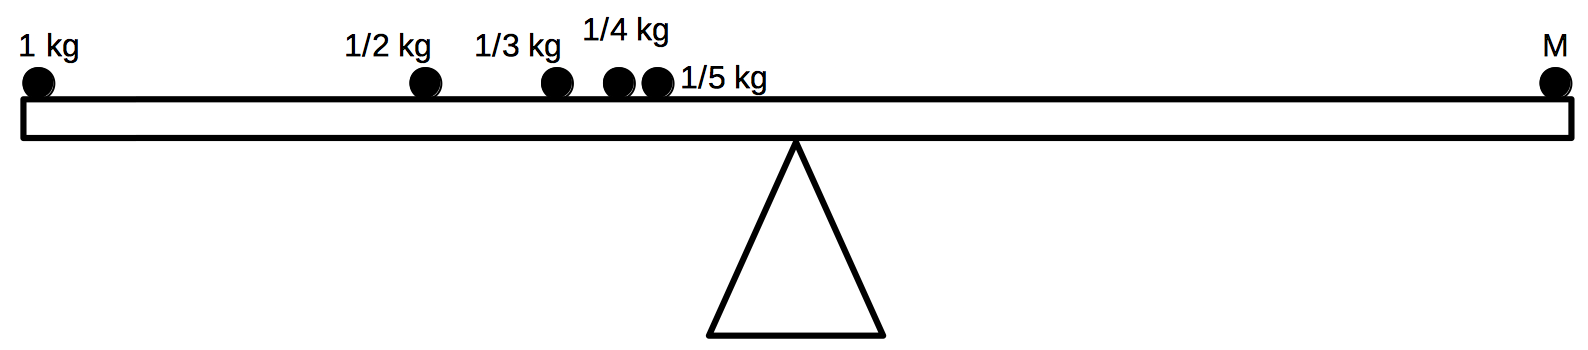
\includegraphics[scale=0.50]{figures/torque/fig1.png}
\end{figure}

\pagebreak \clearpage
